\section{Figures and long tables}
\newpage

\begin{table}[H]

\textbf{\refstepcounter{table}\label{tab:LTP_blast} Table
\arabic{table}.}{$^{15}$N responders BLAST against Living Tree Project}

{\small\begin{tabular}{l>{\itshape}lrl}
    \toprule \\
    \textbf{OTU ID} & \textbf{Species Name} & \textbf{BLAST percent identity} & \textbf{accession} \\
    \midrule
    \multirow{1}{*}{OTU.108} & Caloramator proteoclasticus & 96.94 & X90488 \\ \midrule
\multirow{21}{*}{OTU.14} & Pantoea rwandensis & 99.49 & JF295055 \\  & Pantoea rodasii & 99.49 & JF295053 \\  & Kluyvera intermedia & 99.49 & AF310217 \\  & Kluyvera cryocrescens & 99.49 & AF310218 \\  & Klebsiella variicola & 99.49 & AJ783916 \\  & Klebsiella pneumoniae subsp. rhinoscleromatis & 99.49 & Y17657 \\  & Klebsiella pneumoniae subsp. pneumoniae & 99.49 & X87276 \\  & Erwinia aphidicola & 99.49 & FN547376 \\  & Enterobacter soli & 99.49 & GU814270 \\  & Enterobacter ludwigii & 99.49 & AJ853891 \\  & Enterobacter kobei & 99.49 & AJ508301 \\  & Enterobacter hormaechei & 99.49 & AJ508302 \\  & Enterobacter cloacae subsp. dissolvens & 99.49 & Z96079 \\  & Enterobacter cancerogenus & 99.49 & Z96078 \\  & Enterobacter asburiae & 99.49 & AB004744 \\  & Enterobacter amnigenus & 99.49 & AB004749 \\  & Enterobacter aerogenes & 99.49 & AB004750 \\  & Buttiauxella warmboldiae & 99.49 & AJ233406 \\  & Buttiauxella noackiae & 99.49 & AJ233405 \\  & Buttiauxella izardii & 99.49 & AJ233404 \\  & Buttiauxella agrestis & 99.49 & AJ233400 \\ \midrule
\multirow{2}{*}{OTU.1673} & Clostridium drakei & 95.9 & Y18813 \\  & Clostridium carboxidivorans & 95.9 & FR733710 \\ \midrule
\multirow{2}{*}{OTU.327} & Clostridium hydrogeniformans & 94.92 & DQ196623 \\  & Clostridium amylolyticum & 94.92 & EU037903 \\ \midrule
\multirow{1}{*}{OTU.330} & Clostridium lundense & 96.94 & AY858804 \\ \midrule
\multirow{1}{*}{OTU.342} & Acinetobacter johnsonii & 100.0 & Z93440 \\ \midrule
\multirow{1}{*}{OTU.4037} & Fonticella tunisiensis & 93.85 & HE604099 \\ \midrule
\multirow{4}{*}{OTU.54} & Shigella sonnei & 100.0 & FR870445 \\  & Shigella flexneri & 100.0 & X96963 \\  & Escherichia fergusonii & 100.0 & AF530475 \\  & Escherichia coli & 100.0 & X80725 \\ \midrule
\multirow{2}{*}{OTU.57} & Fonticella tunisiensis & 93.88 & HE604099 \\  & Caloramator proteoclasticus & 93.88 & X90488 \\ \midrule
\multirow{5}{*}{OTU.586} & Vitreoscilla filiformis & 98.48 & HM037993 \\  & Ottowia pentelensis & 98.48 & EU518930 \\  & Ideonella dechloratans & 98.48 & X72724 \\  & Diaphorobacter nitroreducens & 98.48 & AB064317 \\  & Comamonas terrigena & 98.48 & AF078772 \\ \midrule

    \bottomrule
\end{tabular}}{}
\end{table}


\begin{figure}[H]
  \centering
  \caption{Ordination of heavy gradient fractions by Bray-Curtis distances on the basis of OTU content.}
  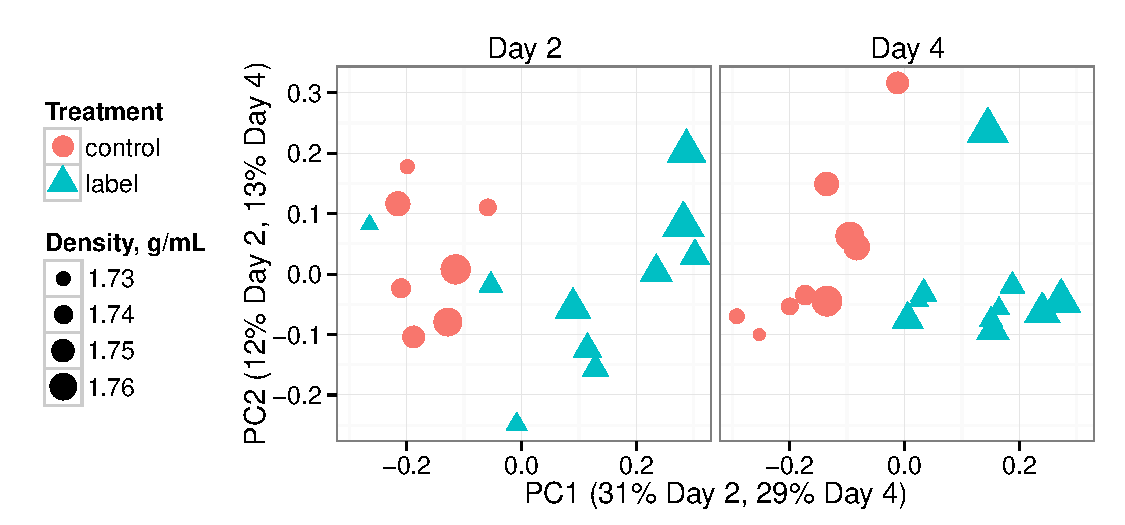
\includegraphics[width=0.85\textwidth]{figures/ordination_heavy/ordination_heavy_day_facet.pdf}
  \label{fig:ord_heavy}
\end{figure}

\begin{figure}[H]
  \centering
  \caption{Phylogenetic trees of OTUs passing sparsity threshold for \textbf{A}
  \textit{Proteobacteria}, \textbf{B} \textit{Acidobacteria} and \textbf{C}
  \textit{Firmicutes}. \textbf{i.} Point denotes OTU is classified as a $^{15}$N
  ``responder''. \textbf{ii.} Heatmap of moderated log$_{2}$ proportion mean
  ratios (labeled:control gradients) for each OTU at each incubation day. High
  values indicate $^{15}$N incorporation. Left most column is day 2, right column
  is day 4. \textbf{iii.} Presence/absence of OTUs
  (black indicates presence) in lichen, light, or dark environmental samples
  \citep{Garcia_Pichel_2013}. \textbf{iv.} Presence/absence of OTUs (black
  indicates presence) in crust and below crust samples \citep{Steven_2013}.}
  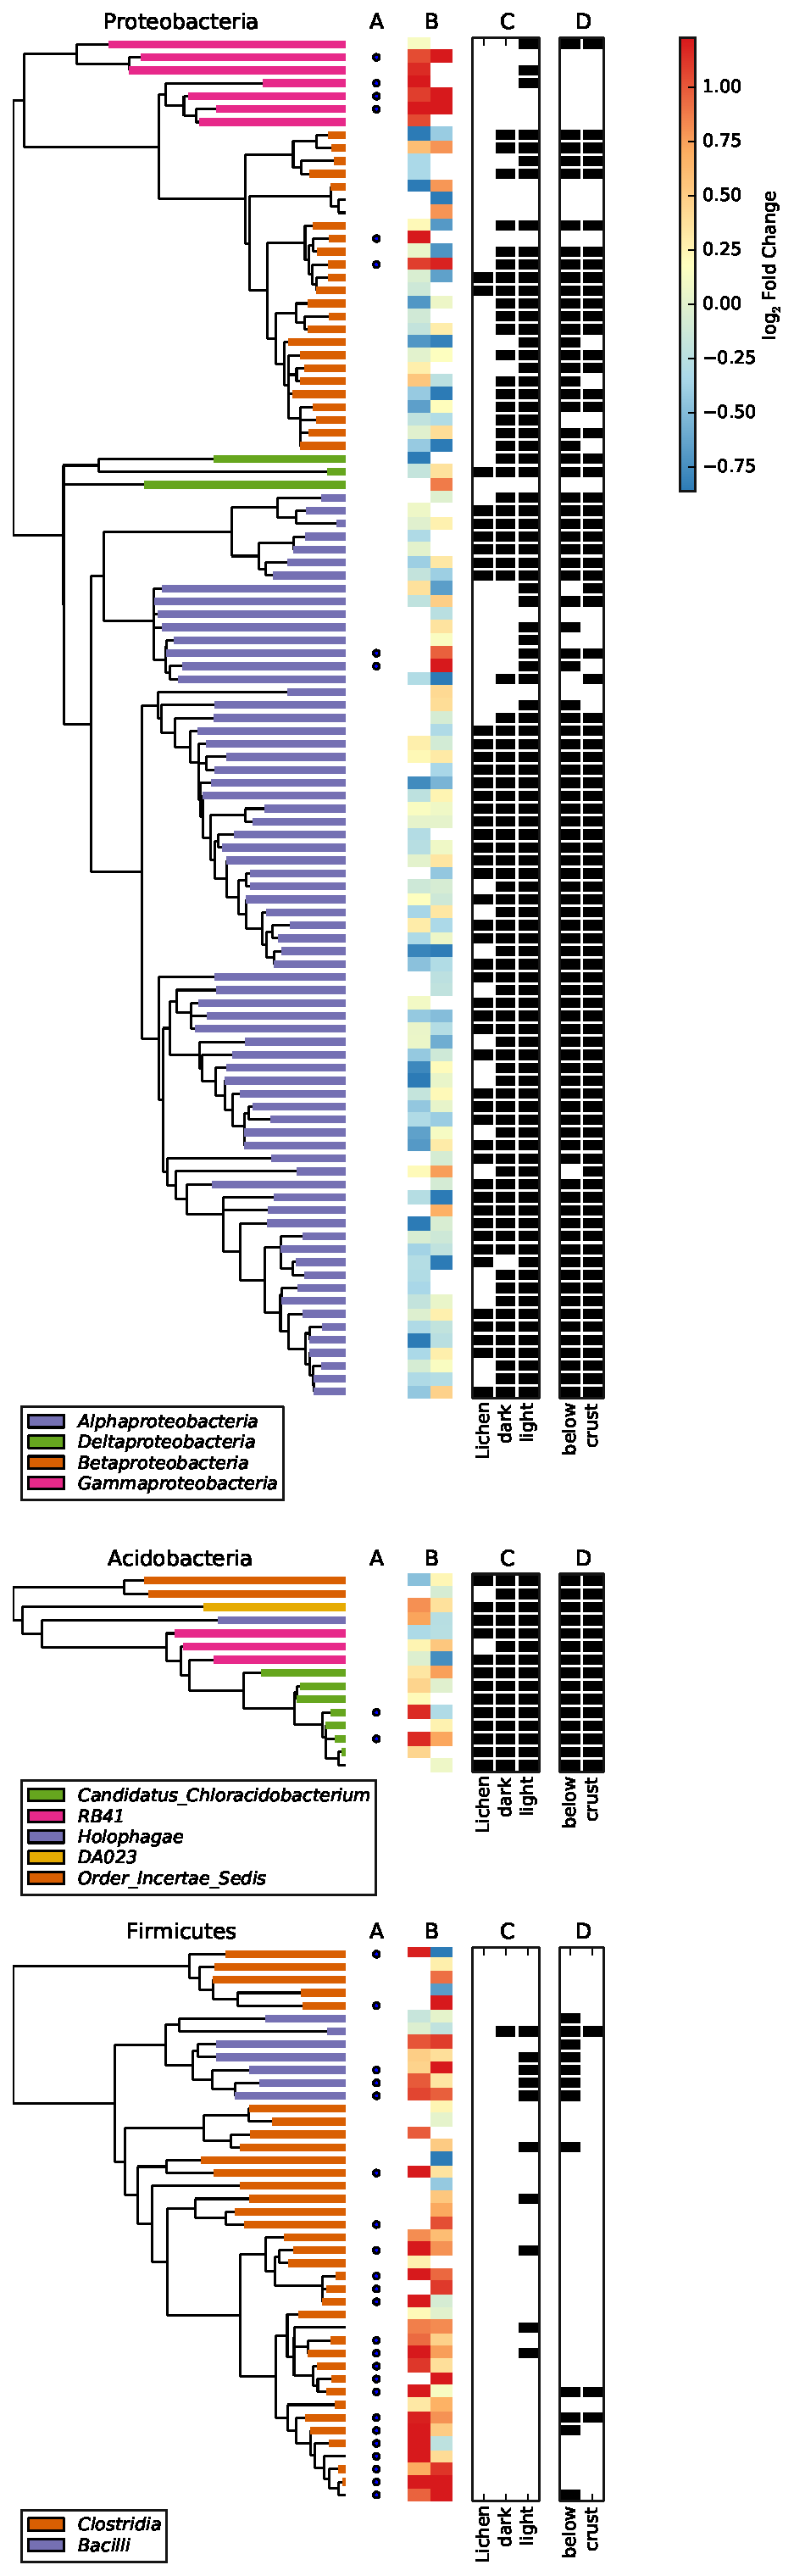
\includegraphics[height=0.95\textheight]{figures/trees/trees.pdf}
    \label{fig:trees}
\end{figure}

\begin{figure}[H]
  \centering
  \caption{Moderated log$_{2}$ of proportion mean ratios for labeled versus
  control gradients (heavy fractions only, densities $>$1.725 g/mL). All OTUs
  passing the sparsity treshold (see methods) at a specific incubation day are
  shown. Red color denotes a proportion mean ratio that has a corresponding
  adjusted p-value below a false discovery rate of 10\% (the null model is that
  the proportion mean is ratio is below 0.25). The horizontal line is the
  proportion mean threshold for the null model, 0.25. The inset figure
  summarizes the taxonomy of OTUs that with proportion mean ratio p-vaules
  under 0.10 for at least one time point.}
  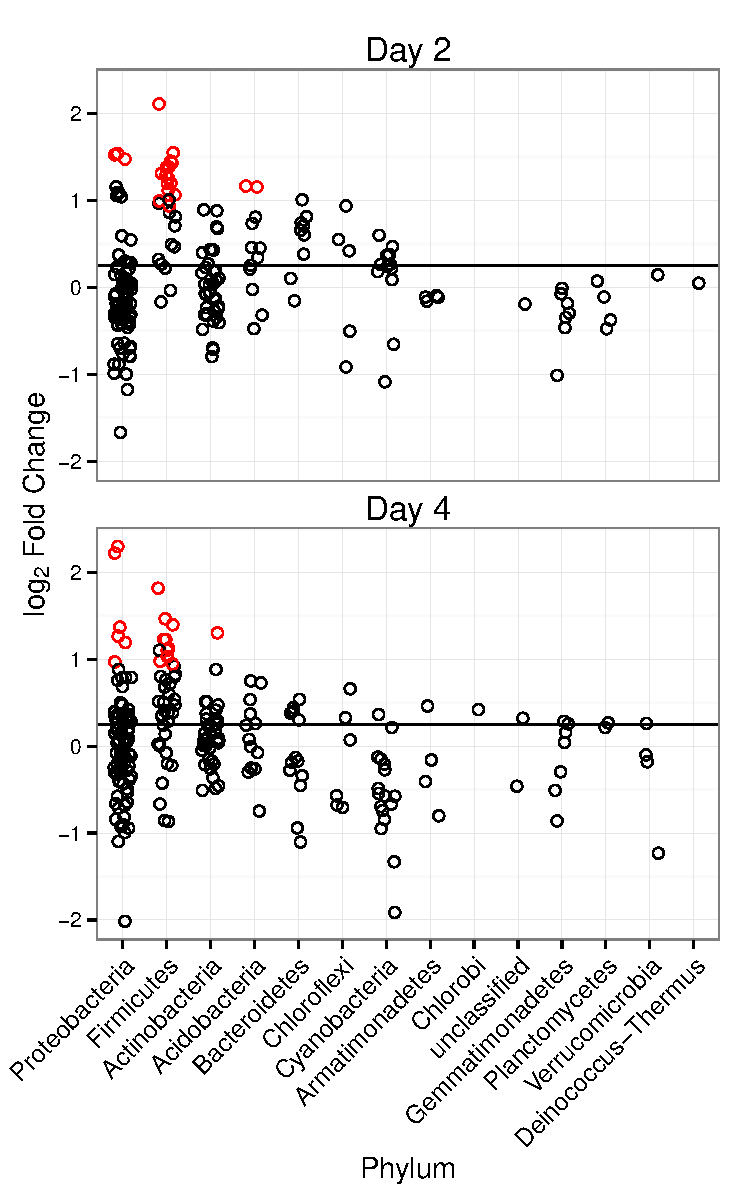
\includegraphics[width=0.5\textwidth]{figures/l2fc/l2fc.pdf}
  \label{fig:l2fc}
\end{figure}

\begin{figure}[H]
  \centering
    \caption{Relative abundance values in heavy fractions (density greater or
    equal to 1.725 g/mL) for the top 10 $^{15}$N "responders" (putative
    diazotrophs, see results for selection criteria of top 10) at each
    incubation day. See Table~\ref{tab:LTP_blast} for BLAST results against 
    the LTP database (release 115). Point area is proportional to CsCl gradient
    fraction density, and color signifies control (red) or labeled (blue)
    treatment.}
    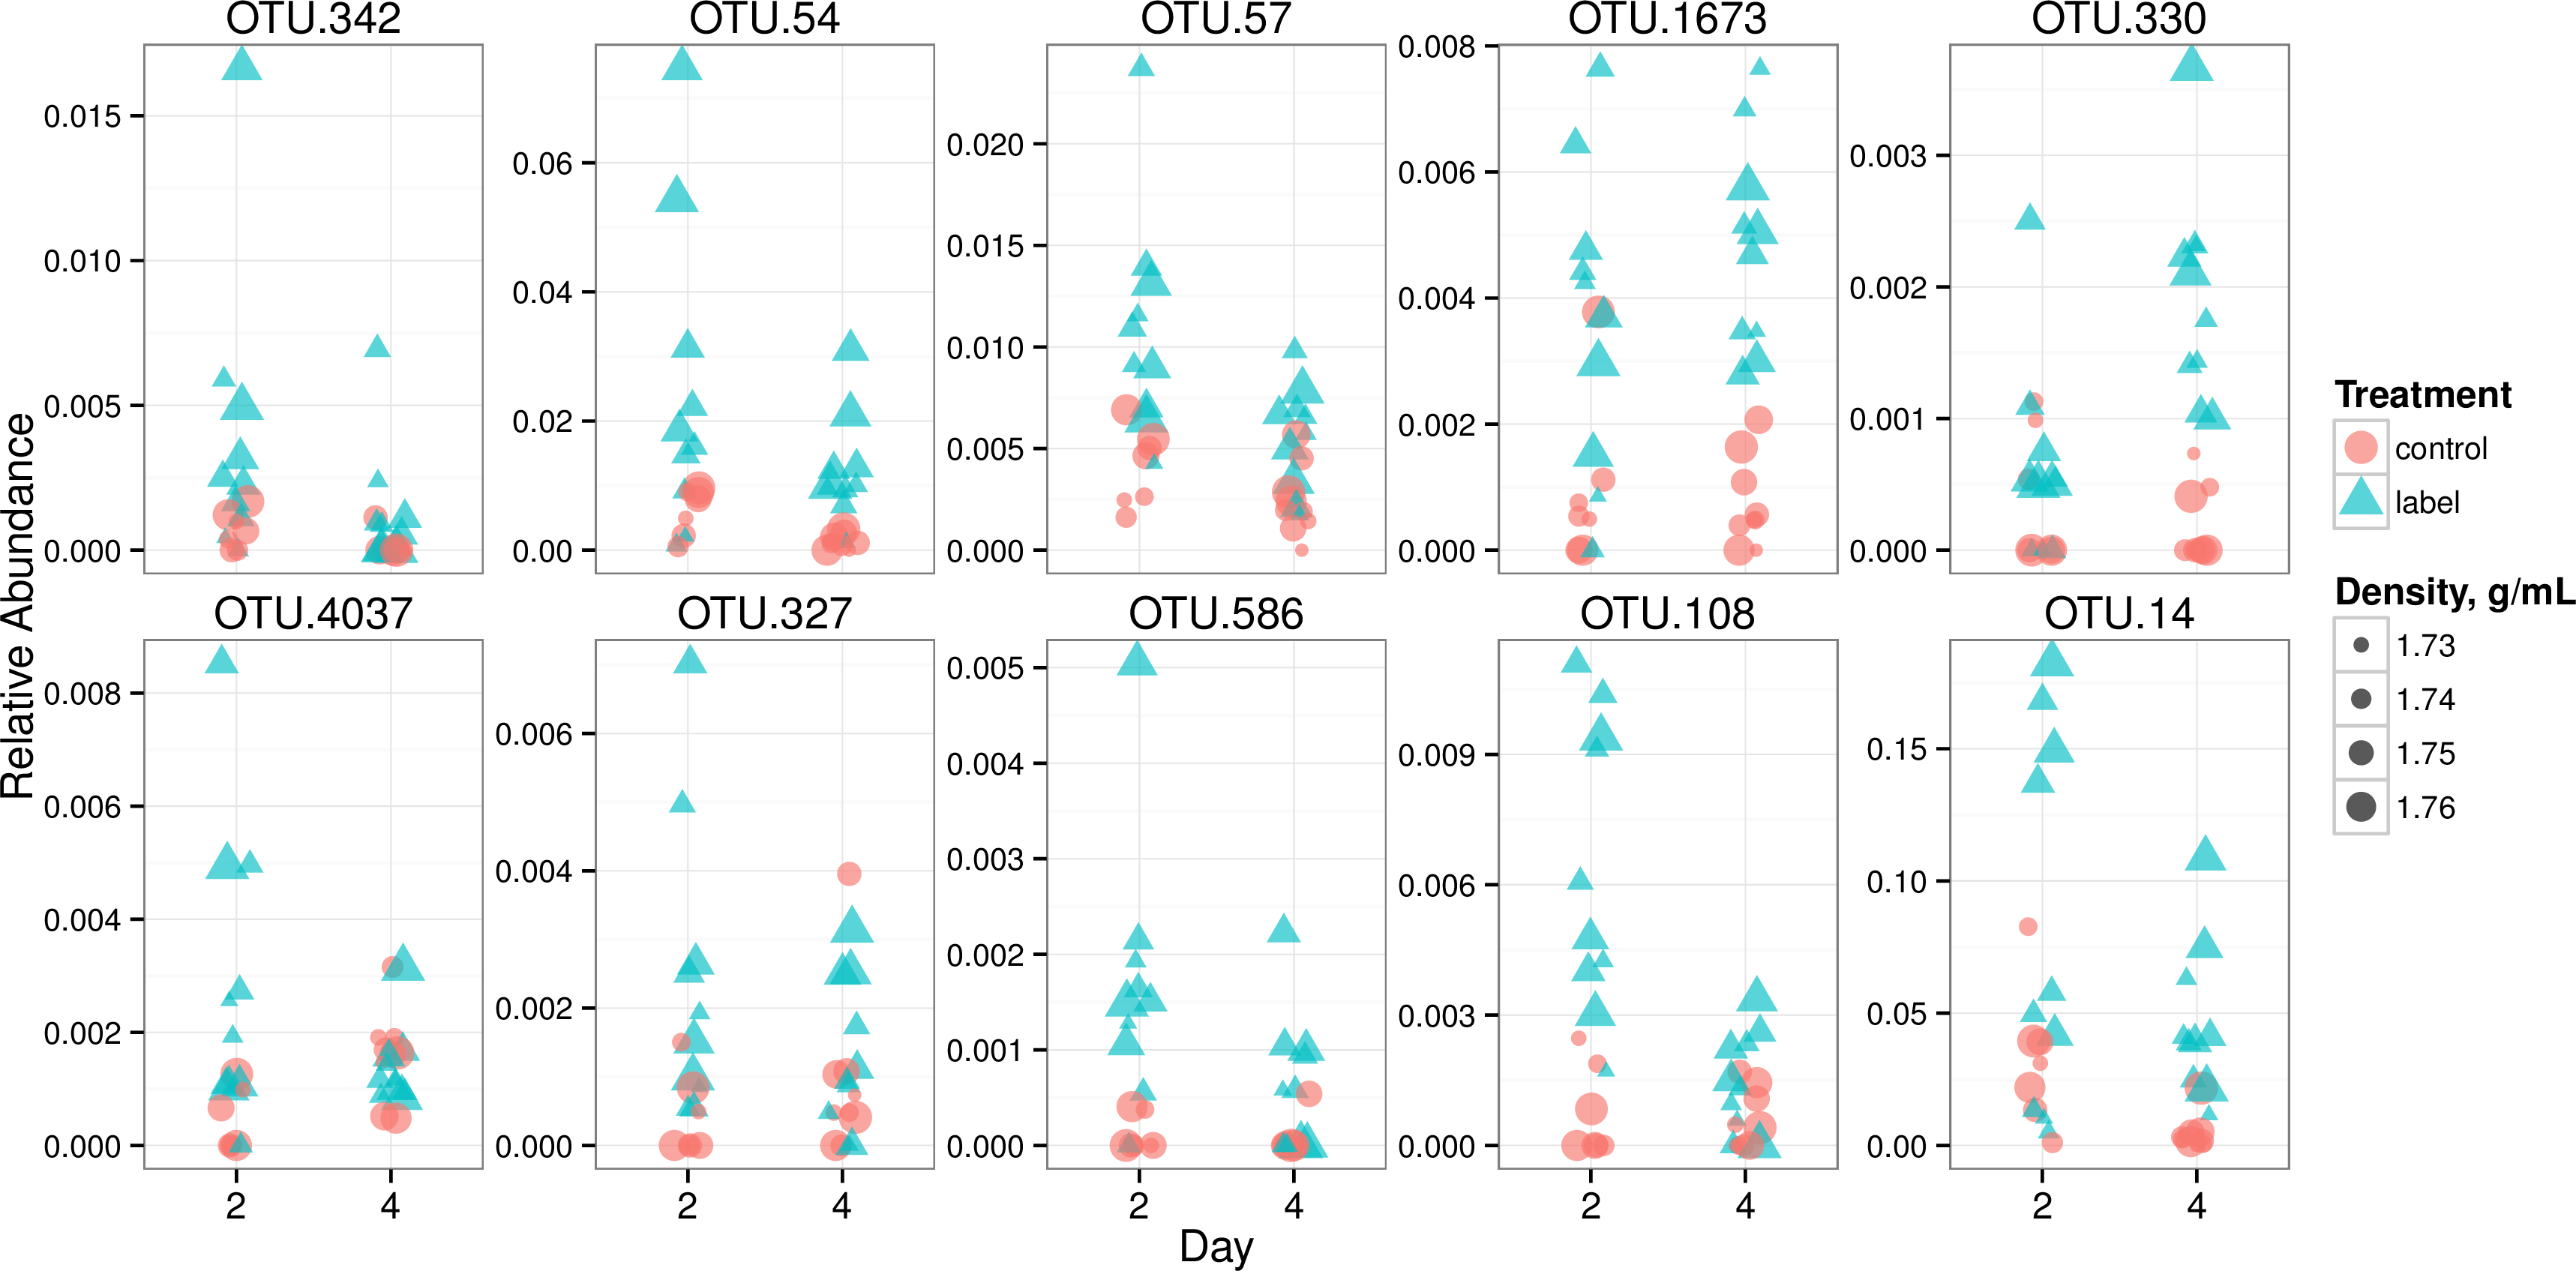
\includegraphics[width=1.0\textwidth]{figures/scatter_heavy_topN2/scatter_heavy_topN.png}
  \label{fig:scatter_heavy}
\end{figure}

\begin{figure}[H]
  \centering
  \caption{See methods for selection criteria for sequences in backbone tree. Edge width is proportional to number of short putative \textit{Clostridiaceae} diazotroph sequences placed at that position. Placement of short sequences can be spread across multiple edges \cite{Matsen_2010}. Reference sequences from cultivars have boxes at tips and full species names. Tips with only accession annotations are from environmental reference sequences.}
    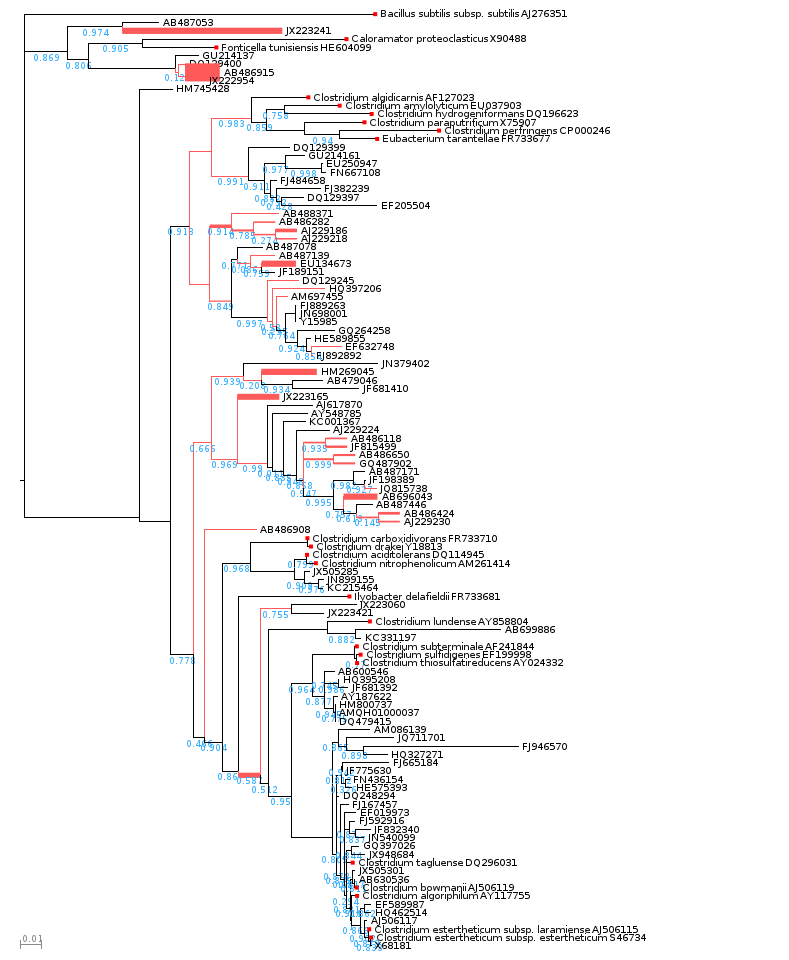
\includegraphics[width=1.0\textwidth]{figures/clost.tree/clost_tree.png}
  \label{fig:clost_tree}
\end{figure}

%\begin{figure}[H]
%  \centering
%    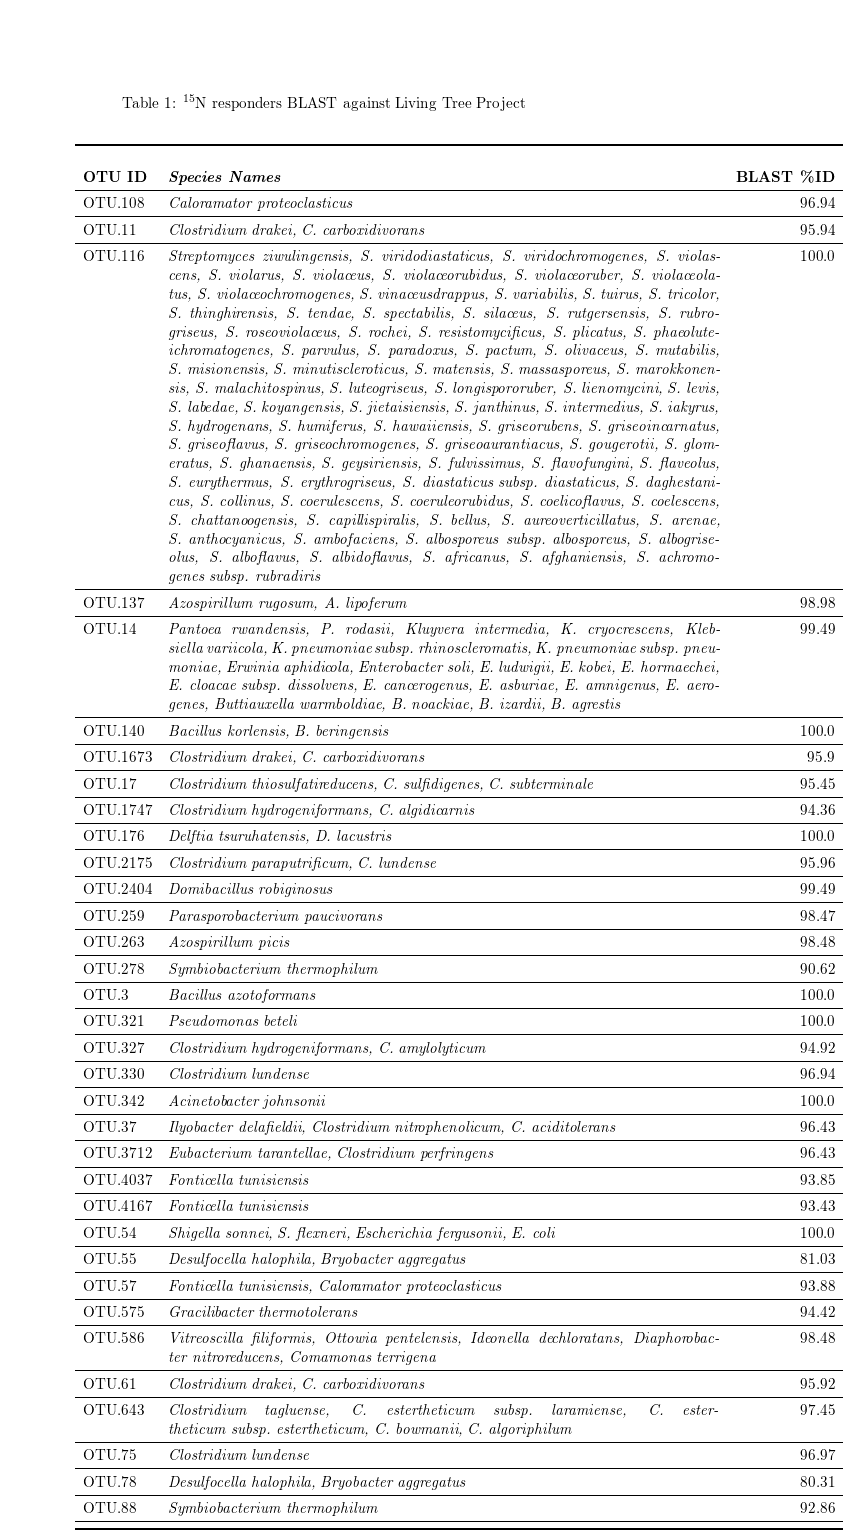
\includegraphics[width=1.0\textwidth]{figures/LTP_blast_table/LTP_blast_table.png}
%  \caption{Replace this text with your caption}
%  \label{tab:LTP_blast}
%\end{figure}
